\section{Proposed exercises}

\subsection{Exercise 1}

In this exercise the classical Cook´s Membrane is proposed to be modelized. Geometry is shown in Figure 57 (mm). The membrane is fixed (encastre) in its left side and a vertical load is distributed along the right side with value $F=1.8\ kN$. The elastic properties of the material are $E=70\ GPa$ and $\nu=0.33$, and its thickness (direction orthogonal to the membrane) is 1 mm. Plane stress hypothesis is considered. We are going to use a structured mesh, subdividing each boundary of the membrane in 16 parts. The elements considered in this exercise are the same ones used in the main practical lesson. 
\begin{figure}[!h]
  \begin{center}
    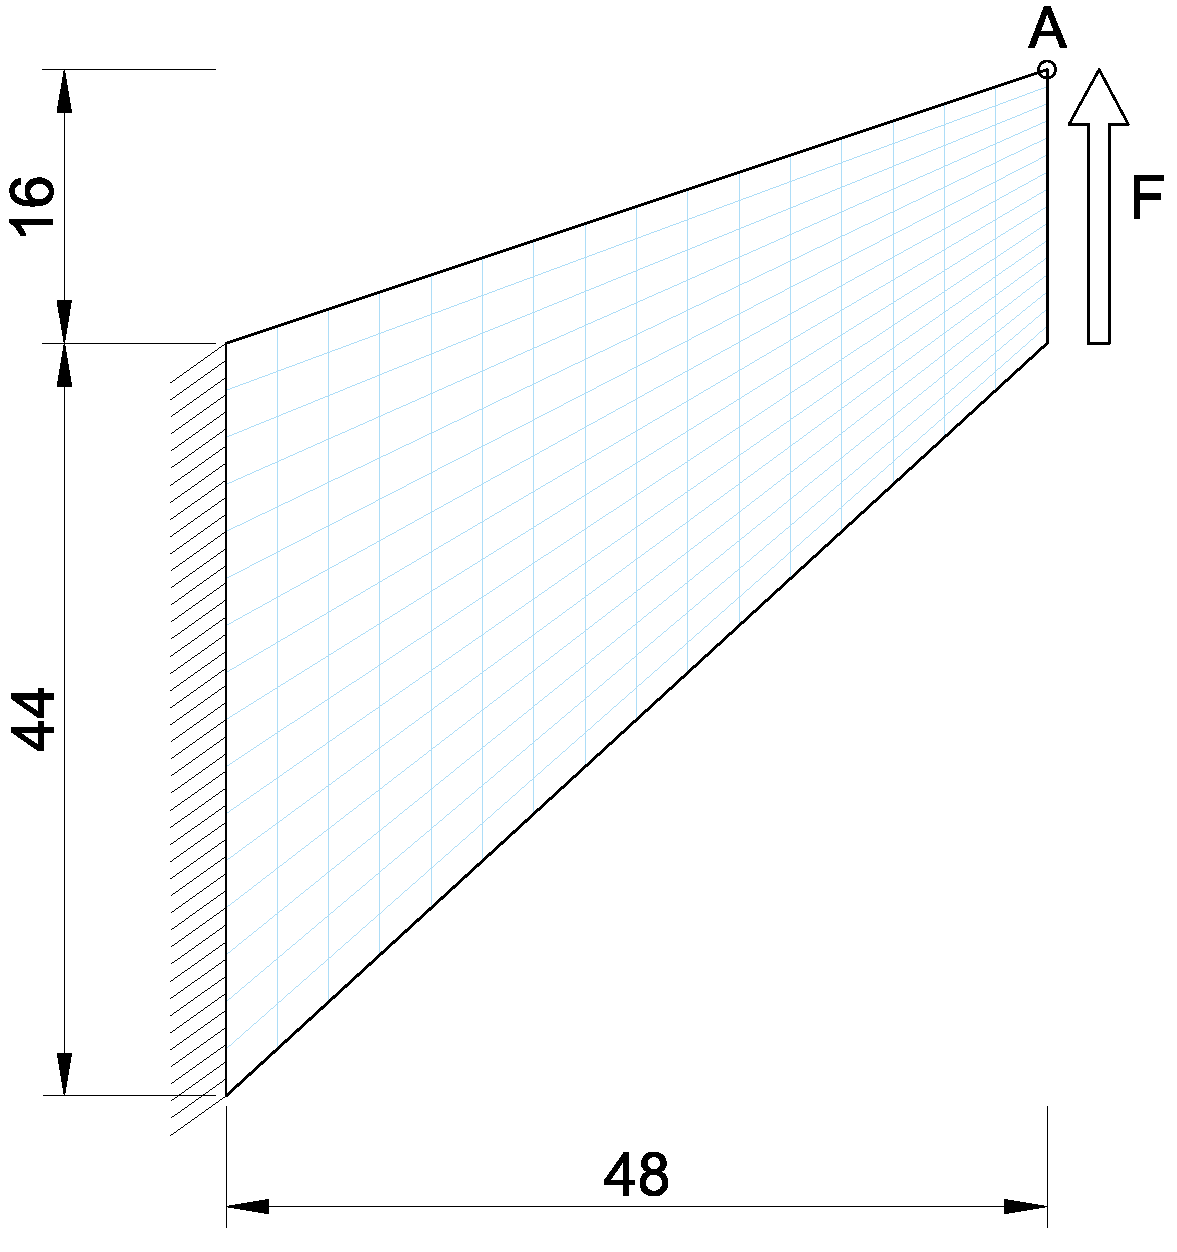
\includegraphics[width=0.55\textwidth]{./body/images/membrana1}
  \end{center}
  \caption{Model description}
  \label{figu120}
\end{figure}
\begin{enumerate}
\item The displacement at point A is:
  \begin{multicols}{4}
  \mybox{A: 0.807 mm} %ok$
\columnbreak
\mybox{B: 1.125 mm}
\columnbreak
\mybox{C: 0.689 mm}
\columnbreak
\mybox{D: 1.333 mm}
  \end{multicols}
\item Maximum value of the reaction in the left side (encastre boundary) is:
  \begin{multicols}{4}
\mybox{A: 1203.0 N}
\columnbreak
\mybox{B: 857.6 N} %ok$
\columnbreak
\mybox{C: 560.3 N}
\columnbreak
\mybox{D: 251.6 N}
  \end{multicols}
\item Maximum value of Von Mises´s stress is:
  \begin{multicols}{4}
\mybox{A: 1321.0 MPa}
\columnbreak
\mybox{B: 854.2 MPa} %ok$
\columnbreak
\mybox{C: 1598.3 MPa}
\columnbreak
\mybox{D: 381.6 MPa}
\end{multicols}
\end{enumerate}



\newpage
\subsection{Exercise 2}

We want to study the mechanical behaviour of the model presented in Fig.~\ref{figu116}, where the circular segments have a radius equal to 1 m. The piece has a state of \textit{plane stress} with the following boundary conditions:
\begin{itemize}
\item All displacements are set to zero in segment $AB$.
\item In segment $EF$ we impose the value of the displacement $u_x^*=0.01$ m.
\item There is a concentrated vertical force of value $F_y=200$ N.
\end{itemize}

The material behaviour is isotropic linear elastic with the elastic modulus $E=1000000$ Pa.~and $\nu=0.25$. In order to build the discretized problem we use a mesh with the following parameters: \textit{quad-dominated, quadratic and with a global size of 0.9}.

\begin{figure}[!h]
  \begin{center}
    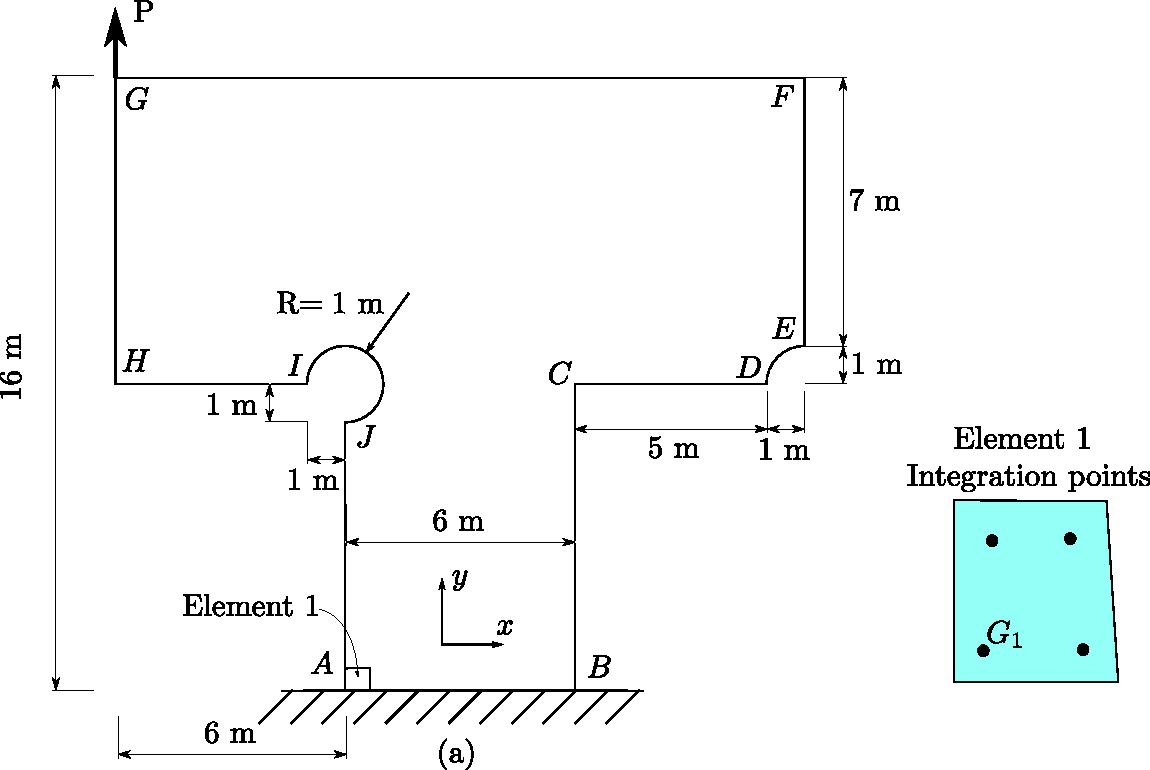
\includegraphics[width=0.65\textwidth]{./body/images/imagen116}
  \end{center}
  \caption{Model description}
  \label{figu116}
\end{figure}

For this model answer the following questions (in this problem you must use some commands we have not explained in the previous example, try to figure it out with the \textit{Help} assistance):



\begin{enumerate}
\item What is the vertical displacement of point H?
  \begin{multicols}{4}
  \mybox{A: 0.0094 m.} %ok$
\columnbreak
\mybox{B: 0.0025 m.}
\columnbreak
\mybox{C: 0.0125 m.}
\columnbreak
\mybox{D: 0.0003 m.}
  \end{multicols}
\item What is the horizontal displacement of point J?
  \begin{multicols}{4}
\mybox{A: 0.0012 m.}
\columnbreak
\mybox{B: 0.0050 m.} %ok$
\columnbreak
\mybox{C: 0.0006 m.}
\columnbreak
\mybox{D: 0.0181 m.}
  \end{multicols}
\item What is the $\sigma_{22}$ component of the stress tensor in the integration point $G_1$ of element 1 (see Figure)?
  \begin{multicols}{4}
  \mybox{A: 710 Pa.} %ok$
\columnbreak
\mybox{B: 1412 Pa.}
\columnbreak
\mybox{C: 172 Pa.}
\columnbreak
\mybox{D: 904 Pa.}
  \end{multicols}
\item What is the maximum value of the maximum principal stress in the path $AF$?
  \begin{multicols}{4}
   \mybox{A: 51 Pa.}
\columnbreak
\mybox{B: 894 Pa.} %ok$
\columnbreak
\mybox{C: 1384 Pa.}
\columnbreak
\mybox{D: 323 Pa.}
\end{multicols}
\item What is the sum of the horizontal reaction forces at the base $AB$?
  \begin{multicols}{4}
   \mybox{A: -231.75 N.}%ok
\columnbreak
\mybox{B: -124.87 N.}
\columnbreak
\mybox{C: -13 N.}
\columnbreak
\mybox{D: -323 N.}
  \end{multicols}
\end{enumerate}
%\hspace{20mm}\hrulefill$\star$\hrulefill\hspace{20mm}
\newpage
\subsection{Exercise 3}
We present here an example that formally is very similar to the
exercise solved in the previous section. It is an L-shaped piece that
is clamped in one of its ends and there is a force distributed in half
of its upper edge. Fig.~\ref{figu115} summarizes the example.


\begin{figure}[!h]
  \begin{center}
    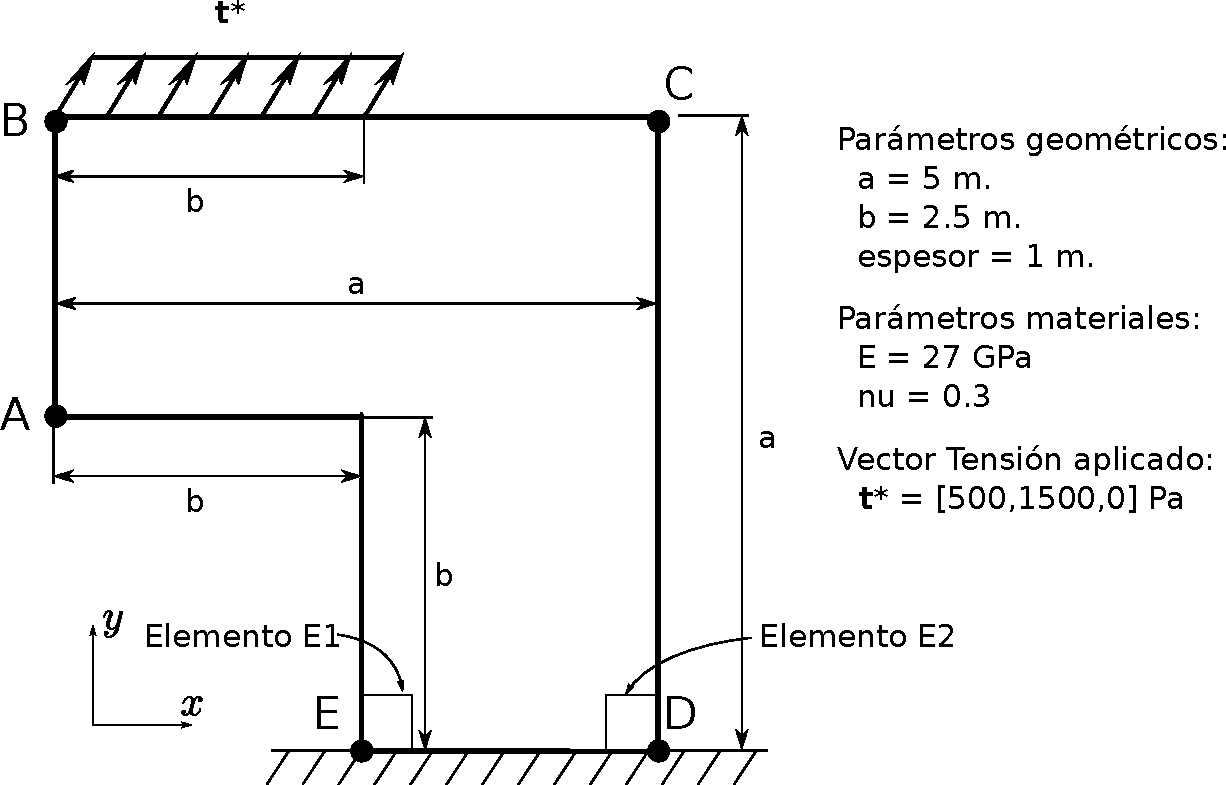
\includegraphics[width=0.65\textwidth]{./body/images/imagen115}
  \end{center}
  \caption{Model description}
  \label{figu115}
\end{figure}

For this model, following the working schema of Section 1, using the
same type of quadrilateral element and a value of element global size
of $0.3$ meters, answer the following questions:



\begin{enumerate}
\item What is the vertical displacement of point B?
  \begin{multicols}{4}
  \mybox{A: 2.821 $\cdot$ 10$^{-6}$ m.}
\columnbreak
\mybox{B: 6.024 $\cdot$ 10$^{-6}$ m.}
\columnbreak
\mybox{C: 2.123 $\cdot$ 10$^{-5}$ m.}
\columnbreak
\mybox{D: 3.254 $\cdot$ 10$^{-9}$ m.}
  \end{multicols}
\item What is the horizontal displacement of point C?
  \begin{multicols}{4}
\mybox{A: 1.627 $\cdot$ 10$^{-6}$ m.}
\columnbreak
\mybox{B: 4.741 $\cdot$ 10$^{-6}$ m.}
\columnbreak
\mybox{C: 2.321 $\cdot$ 10$^{-5}$ m.}
\columnbreak
\mybox{D: 5.237 $\cdot$ 10$^{-9}$ m.}
  \end{multicols}
\item What is the $\sigma_{22}$ component of the stress tensor in the centroid of the element $E1$?
  \begin{multicols}{4}
  \mybox{A: 1782 Pa.}
\columnbreak
\mybox{B: 17413 Pa.}
\columnbreak
\mybox{C: 7174 Pa.}
\columnbreak
\mybox{D: 14904 Pa.}
  \end{multicols}
\item What is the maximum value (in absolute value) of the minimum principal stress $\sigma_3$ in the path $EC$?
  \begin{multicols}{4}
   \mybox{A: -851 Pa.}
\columnbreak
\mybox{B: -8801 Pa.}
\columnbreak
\mybox{C: -1984 Pa.}
\columnbreak
\mybox{D: -3366 Pa.}
  \end{multicols}
\end{enumerate}
%\hspace{20mm}\hrulefill$\star$\hrulefill\hspace{20mm}